\chapter{Formale Grammatiken}
\index{Formale Grammatiken}
% TODO: Chomsky-Hierarchie
%
Die Informatik macht sich Gedanken um die systematische Verarbeitung von Information. Anhand verschiedener Modelle haben wir bereits gesehen, wie wir eine Eingabe nehmen, diese nach Vorschriftsregeln verarbeiten und dann eine Antwort auf das gestellte Anfangsproblem liefern. Dabei haben wir eine wichtige Frage wegfallen lassen: Woher weiß der Algorithmus, ob diese Eingabe valid? Woher weiß die Turingmaschine, dass das---was auf dem Band steht---eine korrekte Eingabe ist, die zu keinem undefinierten Verhalten führt?\footnote{Als Beispiel für undefiniertes Verhalten sei hier die Division durch Null gegeben.}

Das Wortproblem stellt folgende Frage:
\begin{quotation}
  Gegeben sei eine Sprache $S$. Ermittle, ob ein Wort $W$ Teil von $S$ ist oder nicht.
\end{quotation}
%
Wir verwenden die neuen Begriffe \emph{Wort} (String bzw. Zeichenkette) und \emph{Sprache} (synonym Grammatik, Vorschriften über die mögliche Aneinanderreihung von Wörtern). Für diese muss eine Zugehörigkeitsbeziehung ermittelt werden. Führen wir das Konzept der Grammatiken ein.

\section{Eine einfache Grammatik}
%
Gegeben sei eine einfache Grammatik, die genau nur 1 Zeichenkette akzeptieren soll und zwar jene, die nur aus ,,a`` besteht. Diese Sprache sei mit ,,a`` spezifiziert und damit bereits vollständig. Stimmt das Eingabewort $W$ mit der Grammatik ,,a`` überein, wird die Eingabe akzeptiert andernfalls zurückgewiesen. Somit wird das Wortproblem entschieden.

Ein komplexeres Beispiel verwendet mehrere Zeichen: Die Grammatik ,,abb`` akzeptiert genau jene Wörter, die eine Länge 3 und den Aufbau ,,abb`` haben.

Wir möchten unser Konzept erweitern, indem wir Mengen abbilden können. So war es uns bislang nicht möglich eine Grammatik ,,Akzeptiere alle Wörter die nur aus \emph{a}s bestehen`` zu formulieren. Wir führen daher das Konzept der Quantoren ein.

\section{Eine Grammatik mit Wiederholungen}
%
\index{Quantoren (formale Grammatiken)}
Wiederholungen werden durch Symbole mit spezieller Bedeutung repräsentiert. In Tabelle~\ref{tab:quantifiers} werden diese Quantoren vorgestellt. Wir können damit mehr Grammatiken als vorhin definieren.

Gesucht sei folgende Grammatik:
\begin{quote}
  Das Zeichen ,,a`` kann (aber muss nicht) vorkommen. Nachfolgend kommt ein ,,b`` und anschließend beliebig viele ,,c``.
\end{quote}

Der folgende Ausdruck spezifiziert diese Grammatik:
\lstset{language={}, label={lst:regq}, caption={Die Grammatik $\{a^n b c^m | 0\leq n\leq 1, m \geq 0\}$}, frame={single}}
\begin{lstlisting}
a?bc*
\end{lstlisting}

\begin{table}[ht]
 \begin{center}
  \begin{tabular}{cl}
   \hline
    + & Das vorige Zeichen kommt 1--$\infty$ mal vor (,,1-mal oder öfters``) \\
    * & Das vorige Zeichen kommt 0--$\infty$ mal vor (,,beliebig oft``) \\
    ? & Das vorige Zeichen kommt 0--1 mal vor (,,optional``) \\
   \hline
  \end{tabular}
  \caption{Quantoren zur Beschreibung unserer Grammatiken}
  \label{tab:quantifiers}
 \end{center}
\end{table}

\section{Eine Grammatik mit Alternationen}
%
Gesucht sei folgende Grammatik:
\begin{quote}
  Die Zeichenkette beginnt mit ,,Message of the `` und hört entweder mit ,,Day`` oder ,,Month``. Am Ende befindet sich ein Rufzeichen ,,!``.
\end{quote}

Für dieses Problem benötigen wir zwei Konzepte: Einerseits brauchen wir ein exklusives Oder, welches uns eine Option selektiert. Andererseits brauchen wir Bereiche, sodass wir Operatoren nicht nur auf einzelne Zeichen sondern ganze Blöcke anwenden können. Die beiden Konzepte nennen sich Alternation (vertikaler Strich) und Gruppen (runde Klammern). Die Verwendung sollte aus der Lösung hervorgehen.

\lstset{language={}, label={lst:message}, caption={Die Message-Grammatik}, frame={single}}
\begin{lstlisting}
Message of the (Day|Month)!
\end{lstlisting}

\section{Reguläre Ausdrücke}
%
Reguläre Ausdrücke (engl. ,,Regular Expressions``, kurz ,,RegEx``) sind eine Notation, um Grammatiken zu beschreiben. Was vorhin als Grammatik-Beschreibung bezeichnet wurde, ist in Wirklichkeit \emph{einer} von mehreren Wegen eine Grammatik zu formulieren. 

Wir spezifizieren, dass ein ,,Terminal`` ein Zeichen ist, welches in der selben Form in der Ausgabe vorkommt. Wir fassen die Operatoren von regulären Ausdrücken zusammen (Tabelle~\ref{tab:regex_op}).

\begin{table}[ht]
 \begin{center}
  \begin{tabular}{cl}
   \hline
    .     & Ein beliebiges Zeichen \\
 {[}ab{]} & Eines der Zeichen aus $\set{a, b}$ \\
    (ab)  & Fasst die Sequenz ,,ab`` zu einer Gruppe zusammen \\
    a|bc  & Entweder ,,a`` oder ,,bc`` \\
    +     & Das vorige Zeichen kommt 1--$\infty$ mal vor (,,1-mal oder öfters``) \\
    *     & Das vorige Zeichen kommt 0--$\infty$ mal vor (,,beliebig oft``) \\
    ?     & Das vorige Zeichen kommt 0--1 mal vor (,,optional``) \\
   \hline
  \end{tabular}
  \caption{RegEx Operatoren}
  \label{tab:regex_op}
 \end{center}
\end{table}

\subsection{Non-greedy Verhalten}
%
Maschinen, die reguläre Ausdrücke verarbeiten arbeiten unterschiedlich. Alte Implementierungen nutzen Backtracking-Verfahren und neuere Implementierungen besitzen viel mehr Optimierungen. Die wesentliche Frage ist, wie diese Maschinen implementiert sind, da sie das Verhalten der regulären Ausdrücke bestimmen.

Wie sieht es mit dem regulären Ausdruch ,,(.*)(.*)`` und der Eingabe ,,abc`` aus? Greedy-Verhalten bezeichnet das Bestreben eines Ausdrucks, möglichst viel Inhalt zu matchen). Entsprechend würde die erste Punkt-Stern-Kombination die gesamte Eingabe matchen, da sie versucht sich alles zuzuweisen. Non-greedy Verhalten kann man meist durch das Anfügen eines Fragezeichens nach dem Gruppenquantor erreichen. Für unser Beispiel wäre etwa ,,(.*?)(.*)`` sinnvoll, wenn der gesamte String der zweiten Kombination zugewiesen werden soll.

\section{Kontextfreie Grammatiken}
%
Gesucht sei folgende Grammatik:
\begin{quote}
  Die Anzahl der ,,a`` ist gleich der Anzahl von ,,b``. 
\end{quote}

Diese vorgegebene Sprache lässt sich mit einem regulären Ausdruck verarbeiten.
\lstset{language={}, label={lst:eqo}, caption={Anzahl von ,,a`` gleich Anzahl von ,,b``}, frame={single}}
\begin{lstlisting}
(ab)*
\end{lstlisting}

Wir erweitern aber nun unsere Grammatik:
\begin{quote}
  Eine Sequenz von ,,a`` wird von einer Sequenz der gleichen Länge von ,,b`` gefolgt.
\end{quote}

Durch die Vorgabe der Position bekommen wir ein neues Problem. Wir versuchen folgenden regulären Ausdruck:
\lstset{language={}, label={lst:rep}, caption={,,a`` gefolgt von ,,b''}, frame={single}}
\begin{lstlisting}
a*b*
\end{lstlisting}

Das geübte Auge erkennt, dass die Anzahl der erzeugten ,,a`` ungleich der Anzahl von ,,b`` sein kann. Daher repräsentiert dieser reguläre Ausdruck nicht die spezifizierte Grammatik. Wir erkennen, dass die vorliegende Grammatik sich nicht mehr regulär abbilden lässt, sondern kontext-frei ist.

Wir führen zwei neue Notationen ein: Die vorige Grammatik notieren wir jetzt kürzer mit $\set{a^n b^n \mid n \in \mathbb{N}, n \geq 0}$ notieren und damit die textuelle Beschreibung ersetzen. Weiters sei führen wir Ersetzungsregeln ein. Wir geben ein Nonterminal ,,S`` vor und ersetzen das Nonterminal so lange bis wir nur mehr Terminale erhalten. Ab diesem Zeitpunkt wurde von unserer Sprache ein Wort abgeleitet. Das \textdollar{} steht für das leere Wort.
% TODO: fix $ to be \varepsilon

\lstset{language={}, label={lst:cfgsample}, caption={Die kontext-freie Grammatik $\set{a^n b^n}$}, escapechar={}, frame={single}}
\begin{lstlisting}
S ::= aSb | $
\end{lstlisting}

Basierend auf S können wir jetzt beliebige Wörter der Sprache ableiten
\lstset{language={}, label={lst:cfl}, caption={Die Ableitung von ,,aaabbb``}, frame={single}}
\begin{lstlisting}
S
aSb
aaSbb
aaaSbbb
aaa$bbb
aaabbb
\end{lstlisting}

Für kontextfreie Grammatiken dürfen wir Nonterminale definieren, die ersetzt werden. Wir müssen dabei beachten, dass wir auf der linken Seite nur ein Nonterminal verwenden dürfen. % TODO: What are the exact rules?

\section{Kontext-sensitive Grammatik}
%
Eine weitere Ebene stellen die kontext-sensitiven Grammatiken dar. Dazu sei folgende Grammatik zu formulieren:
\[
  \set{a^n b^n c^n \mid n \in \mathbb{N}, n \geq 0}
\]

Unser erster Versuch schlägt fehl: Die Anzahl der ,,a`` und ,,b`` sind äquivalent, aber die ,,c`` sind unabhängig. Folglich kann die formulierte Sprache nicht ihre spezifizierte Grammatik einhalten.
\lstset{language={}, label={lst:cflcsl}, caption={Die kontext-freie Grammatik für ein kontext-sensitives Problem}, frame={single}}
\begin{lstlisting}
S ::= aSbB | $
B ::= Bc
\end{lstlisting}

Wir müssen unsere Grammatik ausbauen und auf der linken Seite sowohl Terminale als auch Non-Terminale verwenden:
\lstset{language={}, label={lst:cslsample}, caption={Die kontext-freie Grammatik $\set{a^n b^n c^n}$}, frame={single}}
\begin{lstlisting}
S ::= aSBH | $
aS ::= aa
aB ::= ab
bB ::= bb
HB ::= BC
bC ::= bc
cC ::= cc
CH ::= CC
\end{lstlisting}

\section{Chomsky-Hierarchie}
%
Wir haben bei diesen Beispielen gesehen, dass gewisse Modelle nicht ausreichen, um Sprachen zu beschreiben. Noam Chomsky hat die Chomsky-Hierarchie formuliert, um Sprachen in Kategorien einzuteilen. Dabei sind reguläre Sprachen die schwächsten Sprachen. Kontextfreie Sprachen stehen über den regulären Sprachen und können auch alle regulären Sprachen abbilden. Am mächtigsten sind die rekursive-aufzählbaren Sprachen, die es etwa erlauben die Anzahl der Rekursionen in den Ersetzungsregeln während der Verarbeitung zu verändern.

Abbildung~\ref{fig:chomsky_hierarchy} visualisiert die Chomsky-Hierarchie.
%
\begin{figure}[ht]
 \begin{center}
  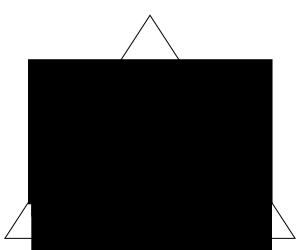
\includegraphics{img/chomsky_hierarchy.pdf}
  \caption{Die Chomsky-Hierarchie}
  \label{fig:chomsky_hierarchy}
 \end{center}
\end{figure}
